\section{Objectives}
Rebuild Lab 20 from PDF pages 81--84, distinguishing combinational propagation/transition times from sequential setup/hold, with successful and failing sweep points.

\section{Specification Mapping}
S denotes simulated checks; D denotes analytical discussion.

\small\begin{longtable}{p{.46\linewidth}p{.30\linewidth}p{.15\linewidth}}\toprule
Requirement and PDF pages & Deck / check & Status \\ \midrule\endhead
Four inverters, 10fF and edge/delay measurements (81,84) & D01/C0 & S \\
Both data-polarity setup times (82--83) & D02; 62 cases & S \\
Both hold times including zero (83) & D03; 102 cases & S \\
Narrow-pulse propagation (84) & D01/C1--5 & S \\
Minimum pulse/release definitions (84) & Discussion & D \\
\bottomrule\end{longtable}\normalsize


\section{Circuit and Design Derivation}
The four inverters use $W_p/W_n/L=3.6/1.8/0.25\,\mu$m and a final 10 fF load. The static DFF follows Fig.20.2(b): four transmission gates and four inverters form master/slave latches, with a 10 fF output load. The master is transparent at low clock and slave at high clock, giving positive-edge capture. Ideal complementary clocks isolate intrinsic timing without clock-inverter skew.
\[t_{PLH/PHL}=t_{out,50\%}-t_{in,50\%},\quad t_r=t_{90\%}-t_{10\%},\quad t_f=t_{10\%}-t_{90\%}.\]
Setup offset is how early the data midpoint precedes the clock midpoint; hold offset is how late it follows. A negative hold value only describes this test, not unrestricted early data changes for arbitrary clock waveforms.

\section{Simulation Setup}
The model is supplied separately on the user's computer. These are 1 V, 27 $^\circ$C teaching conditions; the handout's old-process 2.5 V numbers are not pass thresholds. Actual PrimeSim HSPICE S-2021.09 runs use \texttt{accurate}, \texttt{runlvl=5} and \texttt{.print/.measure} data. Every \texttt{.alter} resets baseline parameters and temperature. All cases completed without errors or failed measurements; model and convergence notices may remain. Public netlists retain only \texttt{* MODEL\_SETUP\_REQUIRED}, with no model path. Full data are under the lab's \texttt{results/}; large files are split by deck and indexed by \texttt{simulation\_data.json}.

Three decks contain 170 cases. The chain uses 5 ps input edges, widths of 1 ns and 100/50/20/10/5 ps, and at most 0.5 ps steps. DFF data/clock edges are 20 ps; the clock midpoint is 1.01 ns. Both data polarities sweep setup from -100 to 200 ps and hold from -300 to 200 ps, in 10 ps steps. DFF simulation lasts 3.5 ns with at most 1 ps steps. Capture at 1.8 ns and retention at 3.0 ns must both satisfy logic0 $\le0.1$ V or logic1 $\ge0.9$ V.

\section{Results and Specification Checks}
\begin{center}\small\begin{tabular}{lrrrrr}\toprule
Width (ps) & $V_{out,pk}$ (V) & $t_{PLH}$ (ps) & $t_{PHL}$ (ps) & $t_r$ (ps) & $t_f$ (ps) \\ \midrule
1000 & 1.1171 & 269.43 & 310.50 & 87.92 & 44.24 \\
100 & 0.7882 & 262.33 & 233.49 & -- & -- \\
50 & 0.0089 & -- & -- & -- & -- \\
20 & 0.0046 & -- & -- & -- & -- \\
10 & 0.0046 & -- & -- & -- & -- \\
5 & 0.0046 & -- & -- & -- & -- \\
\bottomrule\end{tabular}\end{center}

\begin{figure}[htbp]\centering
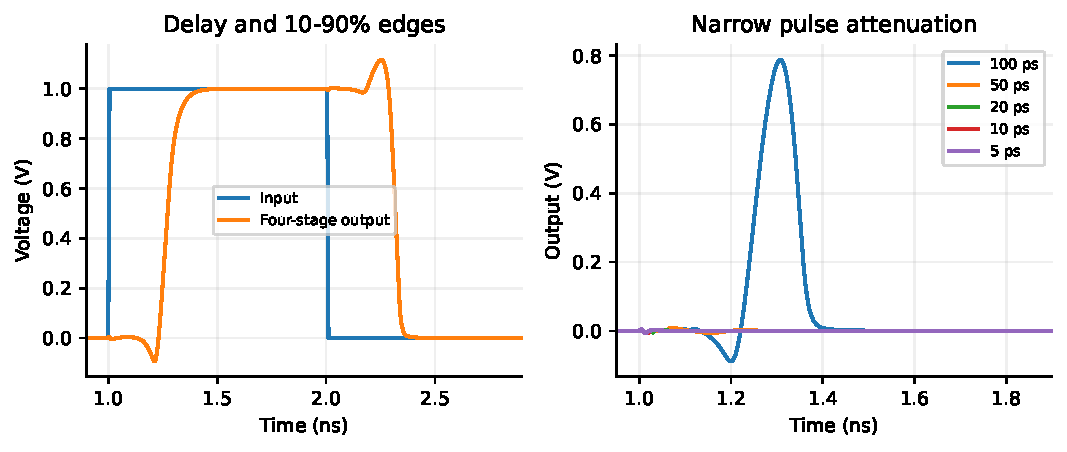
\includegraphics[width=\linewidth]{figures/chain_timing.pdf}
\caption{Four-stage timing and narrow-pulse attenuation. Actual overshoot/undershoot is retained.}
\end{figure}
\begin{center}\small\begin{tabular}{lrrr}\toprule
Check & Captured bit & Failing offset (ps) & Passing offset (ps) \\ \midrule
setup & 0 & 140 & 150 \\
setup & 1 & 110 & 120 \\
hold & 0 & -120 & -110 \\
hold & 1 & -150 & -140 \\
\bottomrule\end{tabular}\end{center}

\begin{figure}[htbp]\centering
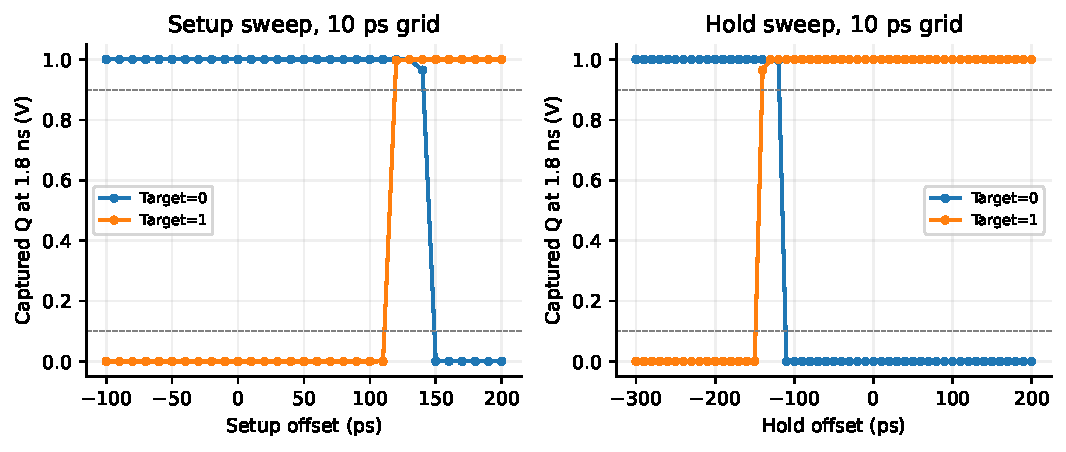
\includegraphics[width=\linewidth]{figures/dff_boundaries.pdf}
\caption{Captured voltage versus offset for both polarities. The pass table also checks retention at 3.0 ns.}
\end{figure}
The worst setup passing point is 150 ps, preceded by failure at 140 ps; the other polarity gives 120/110 ps. The most conservative hold passing point is -110 ps, preceded by failure at -120 ps; the other polarity gives -140/-150 ps. Both polarities pass at zero hold. These are 10 ps-grid boundaries under the declared criterion, not exact continuous-time or clock-to-Q-degradation library limits.

A 100 ps pulse peaks at 0.788 V but misses the 0.9 V valid-high criterion. Pulses of 50 ps or less produce no 50\%-crossing output pulse. A dash denotes a missing crossing, not zero delay.

\section{Discussion}
Finite bandwidth and inertia prevent sufficiently narrow pulses from charging internal nodes to their switching thresholds before the stimulus reverses. Pulses shrink or disappear; a partial voltage excursion near the threshold is not a clean digital pulse. The supplied model with fast ideal sources produces rail excursions; they are retained without claiming reliability ratings.

Minimum pulse width is the high/low duration required to complete a specified clock or set/reset operation. Release/recovery time is the interval from asynchronous-control deassertion to an active clock edge. Fig.20.2(b) has no asynchronous set/reset pin, so these definitions are explained without inventing pin measurements. Setup and hold interact; separate sweeps with other conditions fixed are not a complete two-dimensional timing surface, PVT analysis or metastability MTBF.

\section{Conclusion}
Combinational timing, both setup/hold polarities and the narrow-pulse question have actual results. Worst passing setup/hold points of 150/-110 ps apply to the specified model, clock, load and criterion.
